\documentclass{article}
\usepackage[utf8]{inputenc}

\title{CSE3140 — Lab 5}
\author{Mike Medved, Nithila Annadurai}
\date{November 19th, 2022}

\usepackage{color}
\usepackage{amsthm}
\usepackage{amssymb} 
\usepackage{amsmath}
\usepackage[margin=1in]{geometry} 
\usepackage{listings}
\usepackage{xcolor}
\usepackage{minted}
\usepackage{hyperref}
\usepackage{graphicx}

\hypersetup{
    colorlinks=true,
    linkcolor=blue,
    linkbordercolor={0 0 1}
}

\usemintedstyle{emacs}
% \setmonofont{JetBrains Mono}

\begin{document}

\maketitle

\section*{Deliverables}

\subsection*{Part 1}

Below are the various fields displayed on the main dashboard of the Pineapple we used to conduct the lab, followed by a screenshot of the main dashboard itself.

\begin{table}[!htb]
    \begin{tabular}{|l|l|}
    \hline
    \textbf{Setting}  & \textbf{Explanation}                                                                     \\ \hline
    System Status     & Displays the current CPU and RAM usage percentages                                       \\ \hline
    Disk Usage        & Displays the current disk usage percentage                                               \\ \hline
    Connected Clients & Displays each client that is currently, and was previously associated with the Pineapple \\ \hline
    SSIDs Collected   & Displays all SSIDs collected by the Pineapple since bootup                               \\ \hline
    Campaigns         & Displays a list of current campaigns, including their status, types, and names           \\ \hline
    Notifications     & Displays all status notifications collected by the Pineapple regarding it's operation(s) \\ \hline
    \end{tabular}
\end{table}

\begin{align*}
    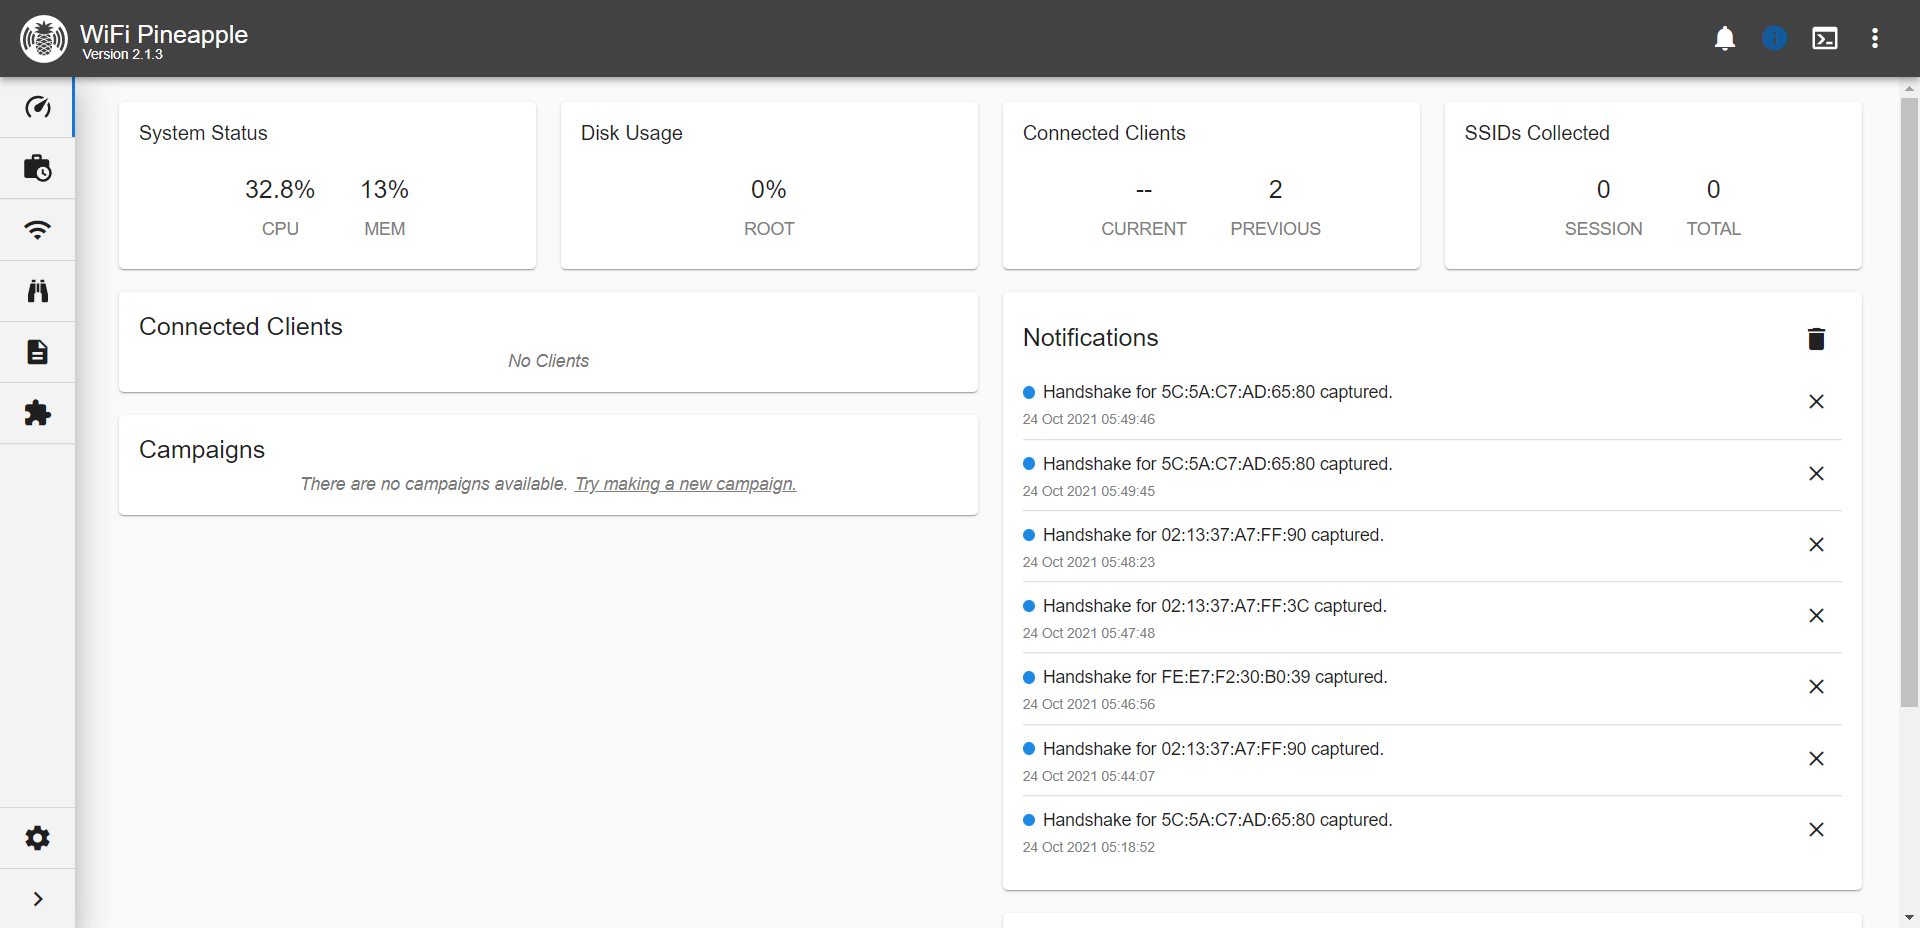
\includegraphics[width=1.0\textwidth]{assets/q1.png}
\end{align*}

\newpage
\subsection*{Part 2}

Below are the various fields found on the Recon dashboard of the Pineapple we used to conduct the lab, followed by screenshots of the dashboard.

\begin{table}[!htb]
    \begin{tabular}{|l|l|l|}
    \hline
    \textbf{Page}       & \textbf{Field}       & \textbf{Explanation}                                                                                                                                                              \\ \hline
    \textbf{Scanning}   & Wireless Landscape   & \begin{tabular}[c]{@{}l@{}}Displays a pie-chart containing the number APs, clients,\\ and unassociated clients\end{tabular}                                                       \\ \hline
                        & Channel Distribution & Displays channel frequencies picked up by the Pineapple's antennas                                                                                                                \\ \hline
                        & Handshakes           & Displays the number of handshakes captured during a Recon scan                                                                                                                    \\ \hline
                        & Previous Scans       & Displays the date and information regarding previous Recon scans                                                                                                                  \\ \hline
                        & Access Points        & \begin{tabular}[c]{@{}l@{}}Displays information regarding detected APs (SSID, MAC, OUI, clients,\\ security, MFP, WPS, channel, signal, and first + last seen times)\end{tabular} \\ \hline
                        & Clients              & \begin{tabular}[c]{@{}l@{}}Displays information regarding all detected clients during scans (IP, MAC,\\ time of connection)\end{tabular}                                          \\ \hline
    \textbf{Handshakes} & Page Information     & \begin{tabular}[c]{@{}l@{}}Displays information regarding captured WPA handshakes (BSSID, client,\\ source, type, time since capture, message1, message2)\end{tabular}            \\ \hline
    \end{tabular}
\end{table}

\begin{align*}
    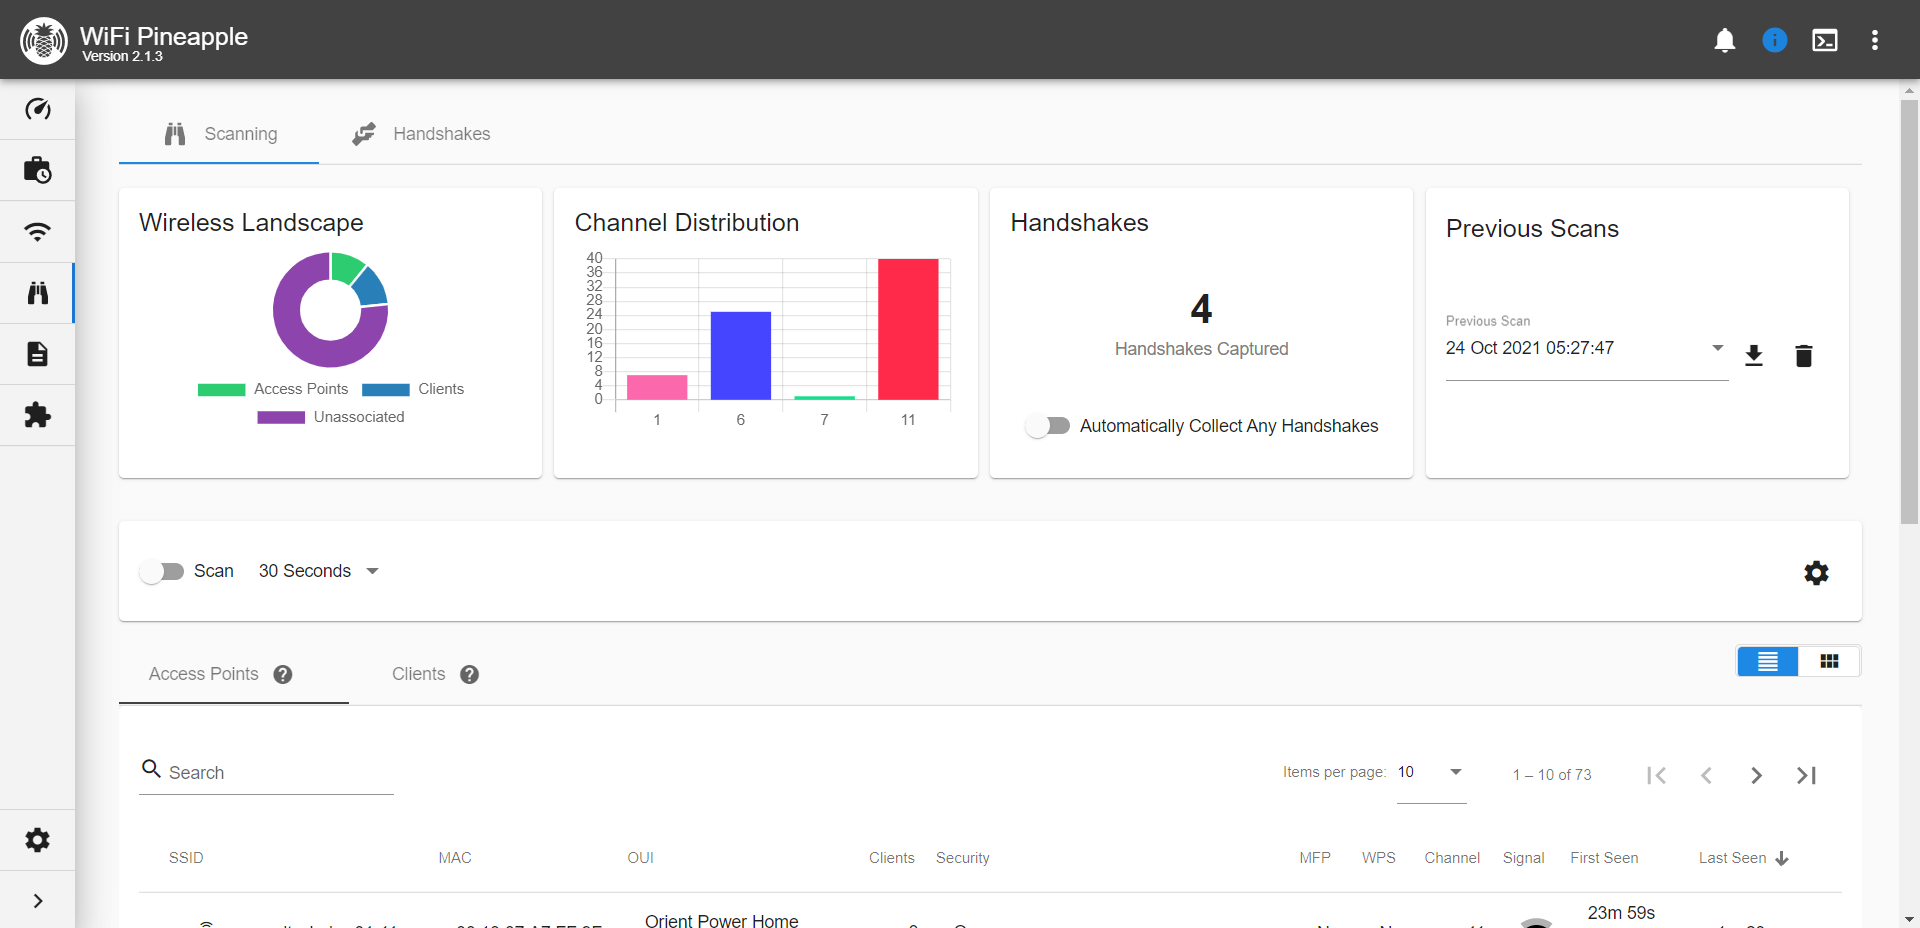
\includegraphics[width=1.0\textwidth]{assets/q2-1.png} \\
\end{align*}

\newpage
\begin{align*}
    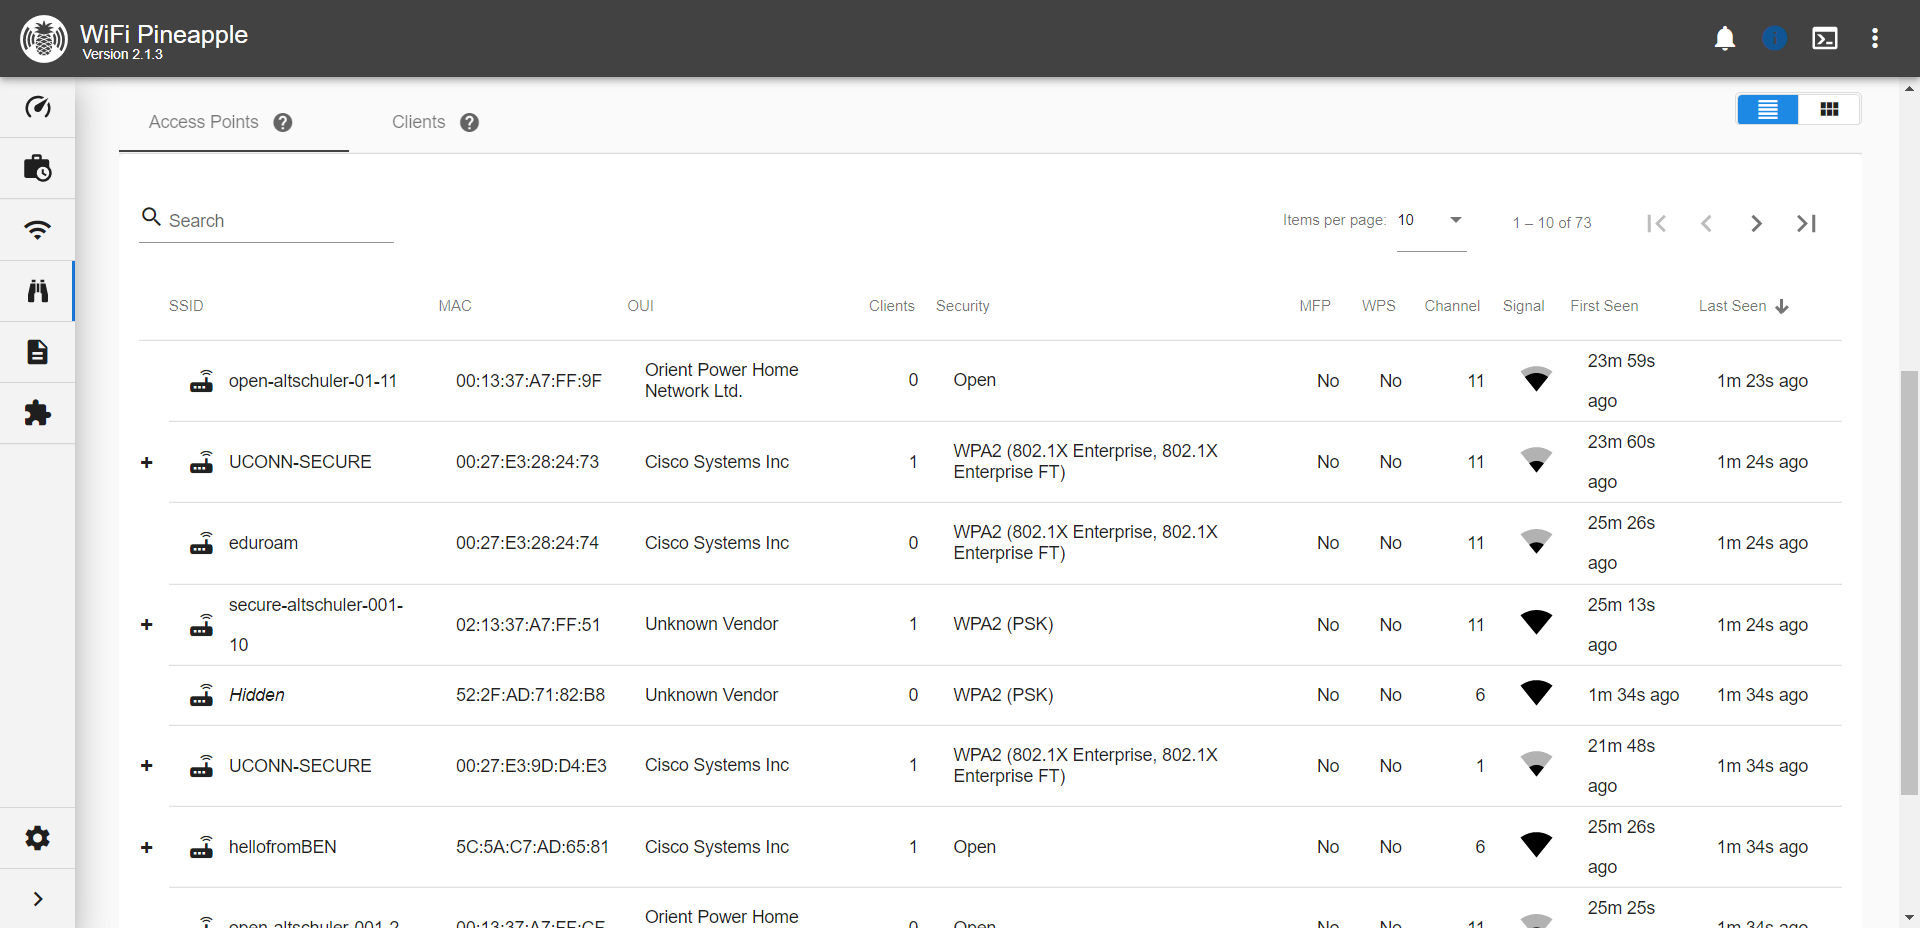
\includegraphics[width=1.0\textwidth]{assets/q2-2.png} \\
    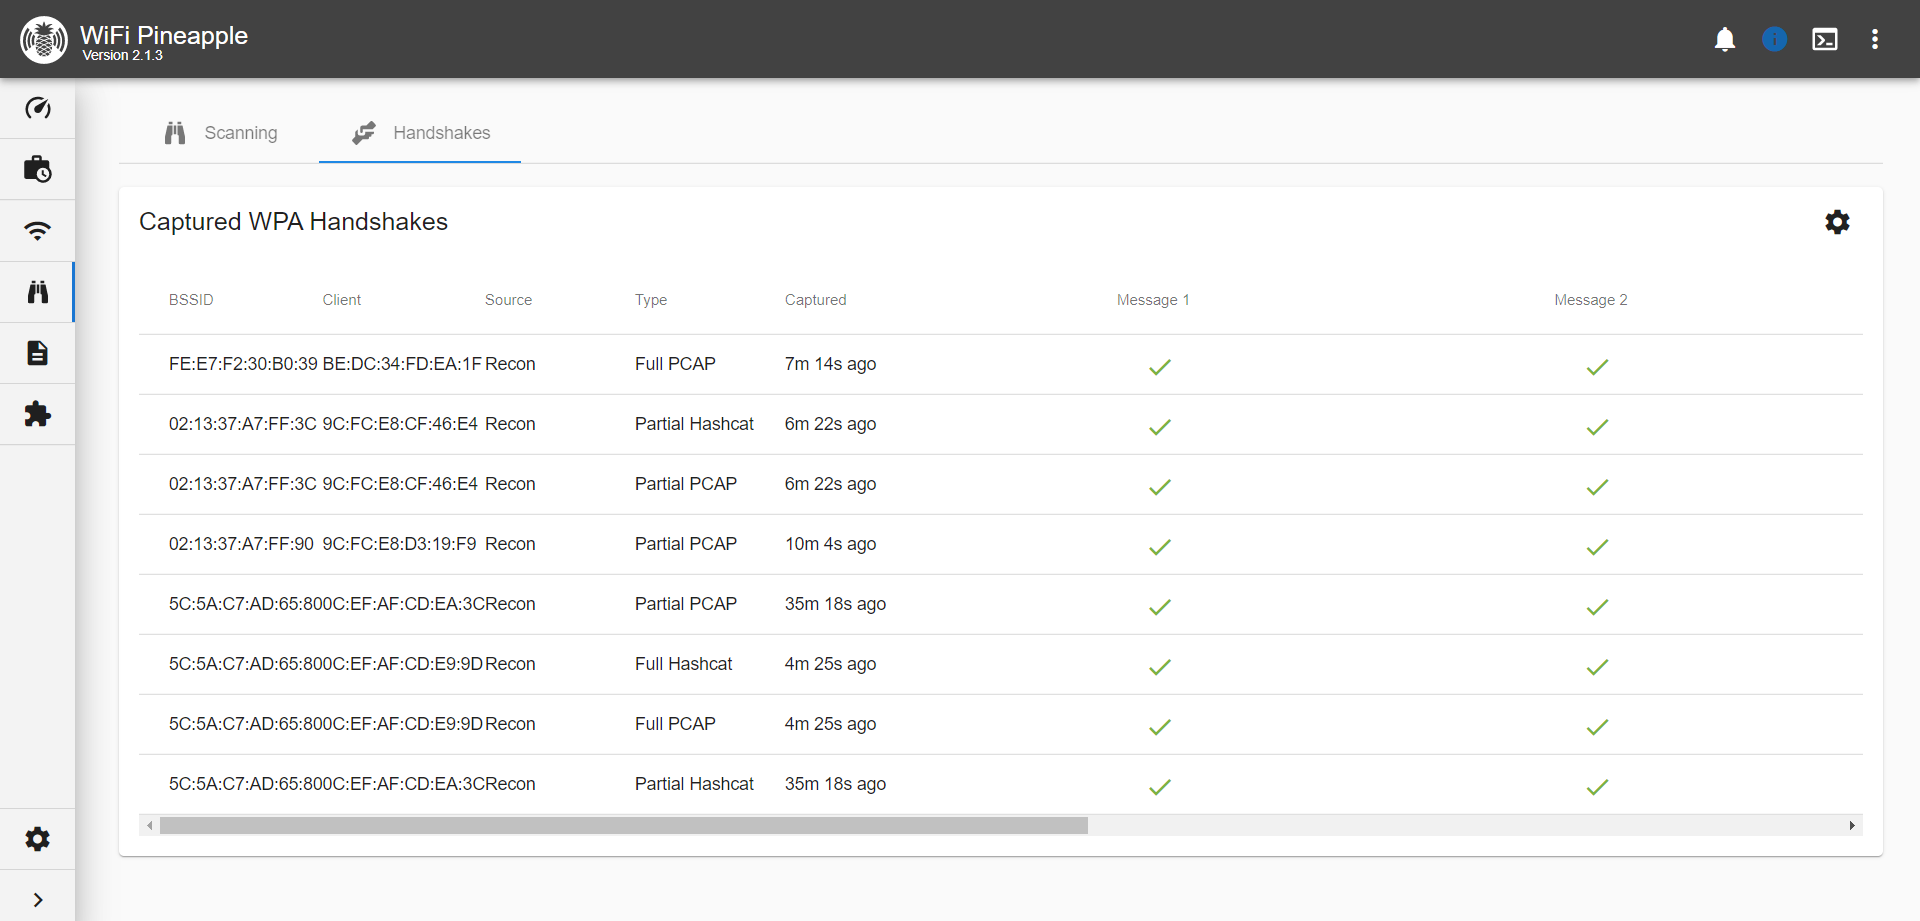
\includegraphics[width=1.0\textwidth]{assets/q2-3.png}
\end{align*}

\newpage
\subsection*{Part 3}

For this question, we were able to see the access point created by personal hotspot on one of our phones:

\begin{align*}
    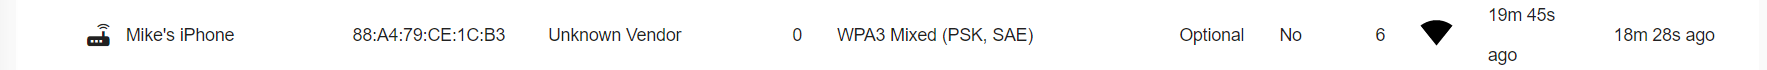
\includegraphics[width=1.0\textwidth]{assets/q3-1.png}
\end{align*}

$\hfill \break$
From the Recon's scanning tab, we were unable to see the users connected to this AP, nor any other access point. This is by design, as the Pineapple should not be able to see the clients associated to unsecured APs, in which case the hotspot was using WPA3 security. The ``cse3140" network was also visible during our scans, and we could see that it was using WPA2 security.

$\hfill \break$
We also managed to capture some handshakes for devices connecting to our vulnerable network, as shown below:

\begin{align*}
    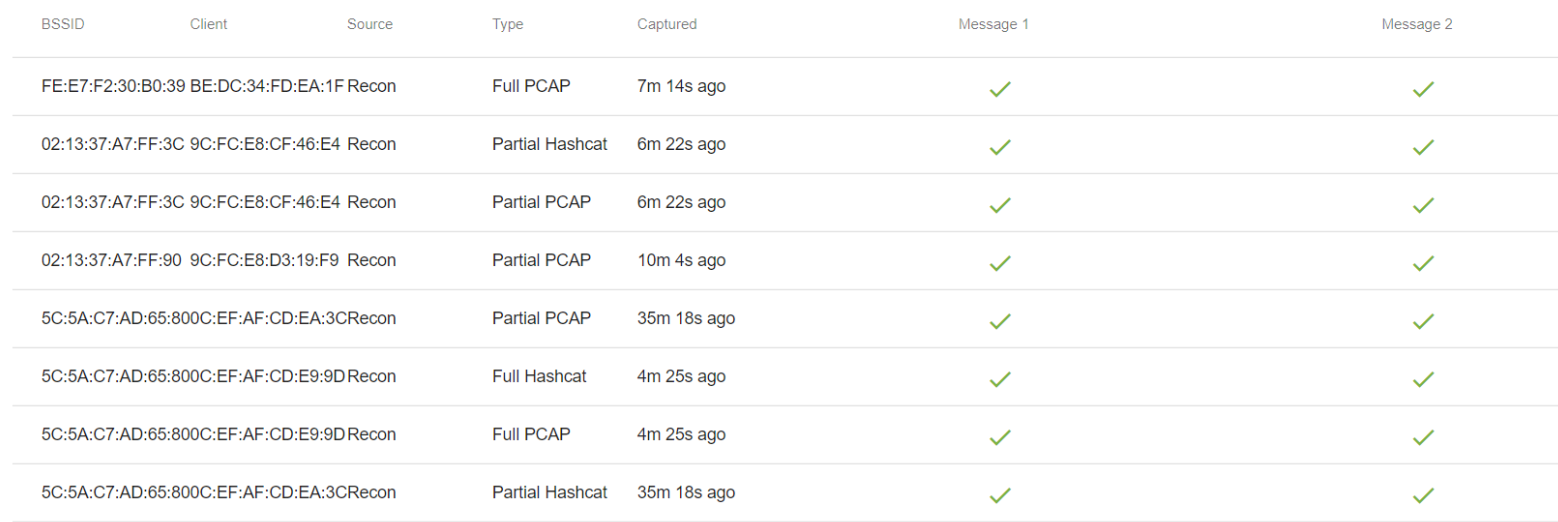
\includegraphics[width=1.0\textwidth]{assets/q3-2.png}
\end{align*}

$\hfill \break$
\begin{table}[!htb]
    \begin{tabular}{|l|l|}
    \hline
    \textbf{Field} & \textbf{Explanation}                                                                     \\ \hline
    BSSID          & The BSSID of the client (as it refers to APs) is essentially it's MAC address            \\ \hline
    Client         & The client fields refers to the client whose handshake has been captured                 \\ \hline
    Source         & The source fields refers to the source of the capture, in this case the Recon module     \\ \hline
    Type           & The type refers to the type of handshake that has been captured, and is available        \\ \hline
    Captured       & The captured field refers to the time since the handshake has been captured              \\ \hline
    Message1       & This boolean field refers to whether or not the Message1 from the handshake was captured \\ \hline
    Message2       & This boolean field, as with the last one, yields whether or not Message 2 was captured   \\ \hline
    \end{tabular}
\end{table}

\newpage
\subsection*{Part 4}

For devices connected to our vulnerable network, we were able to capture unprotected HTTP traffic to the banking website, as shown below:

\begin{align*}
    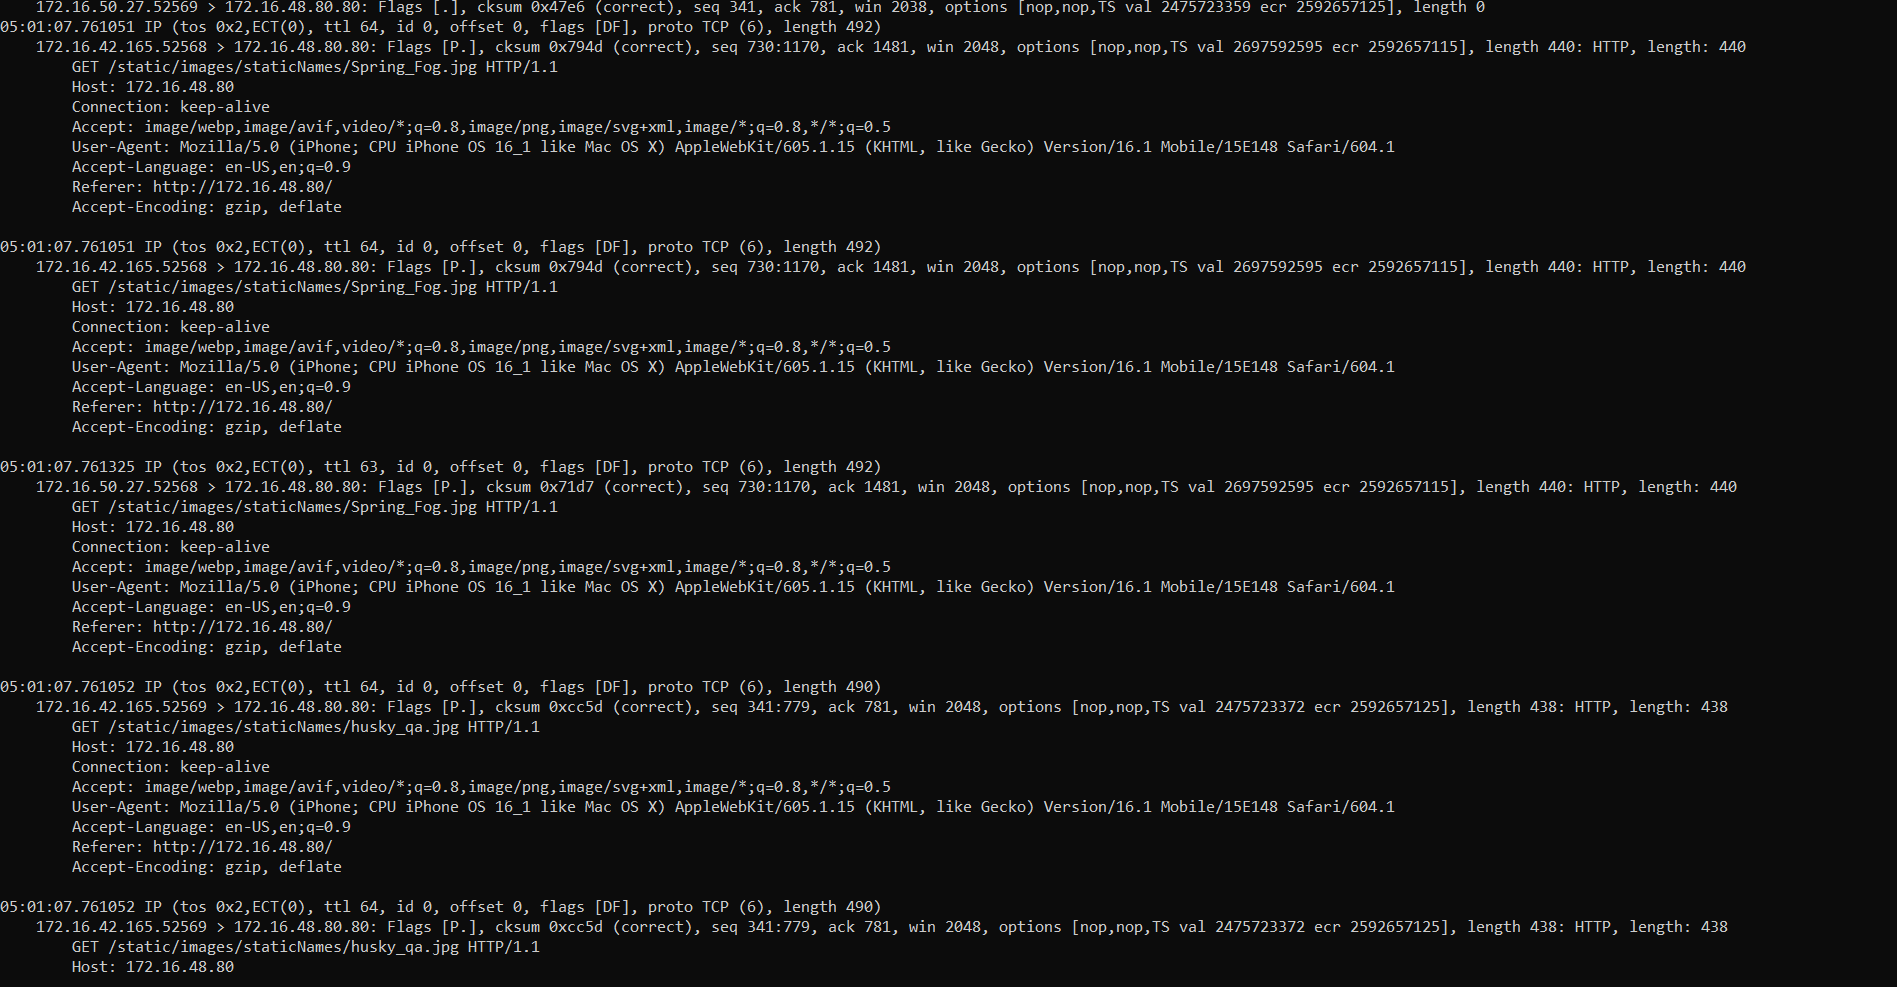
\includegraphics[width=1.0\textwidth]{assets/q4.png}
\end{align*}

\newpage
\subsection*{Part 5}

Similarly, we were also able to observe unprotected HTTP traffic moving along our secure network in much the same way, as shown below:

\begin{align*}
    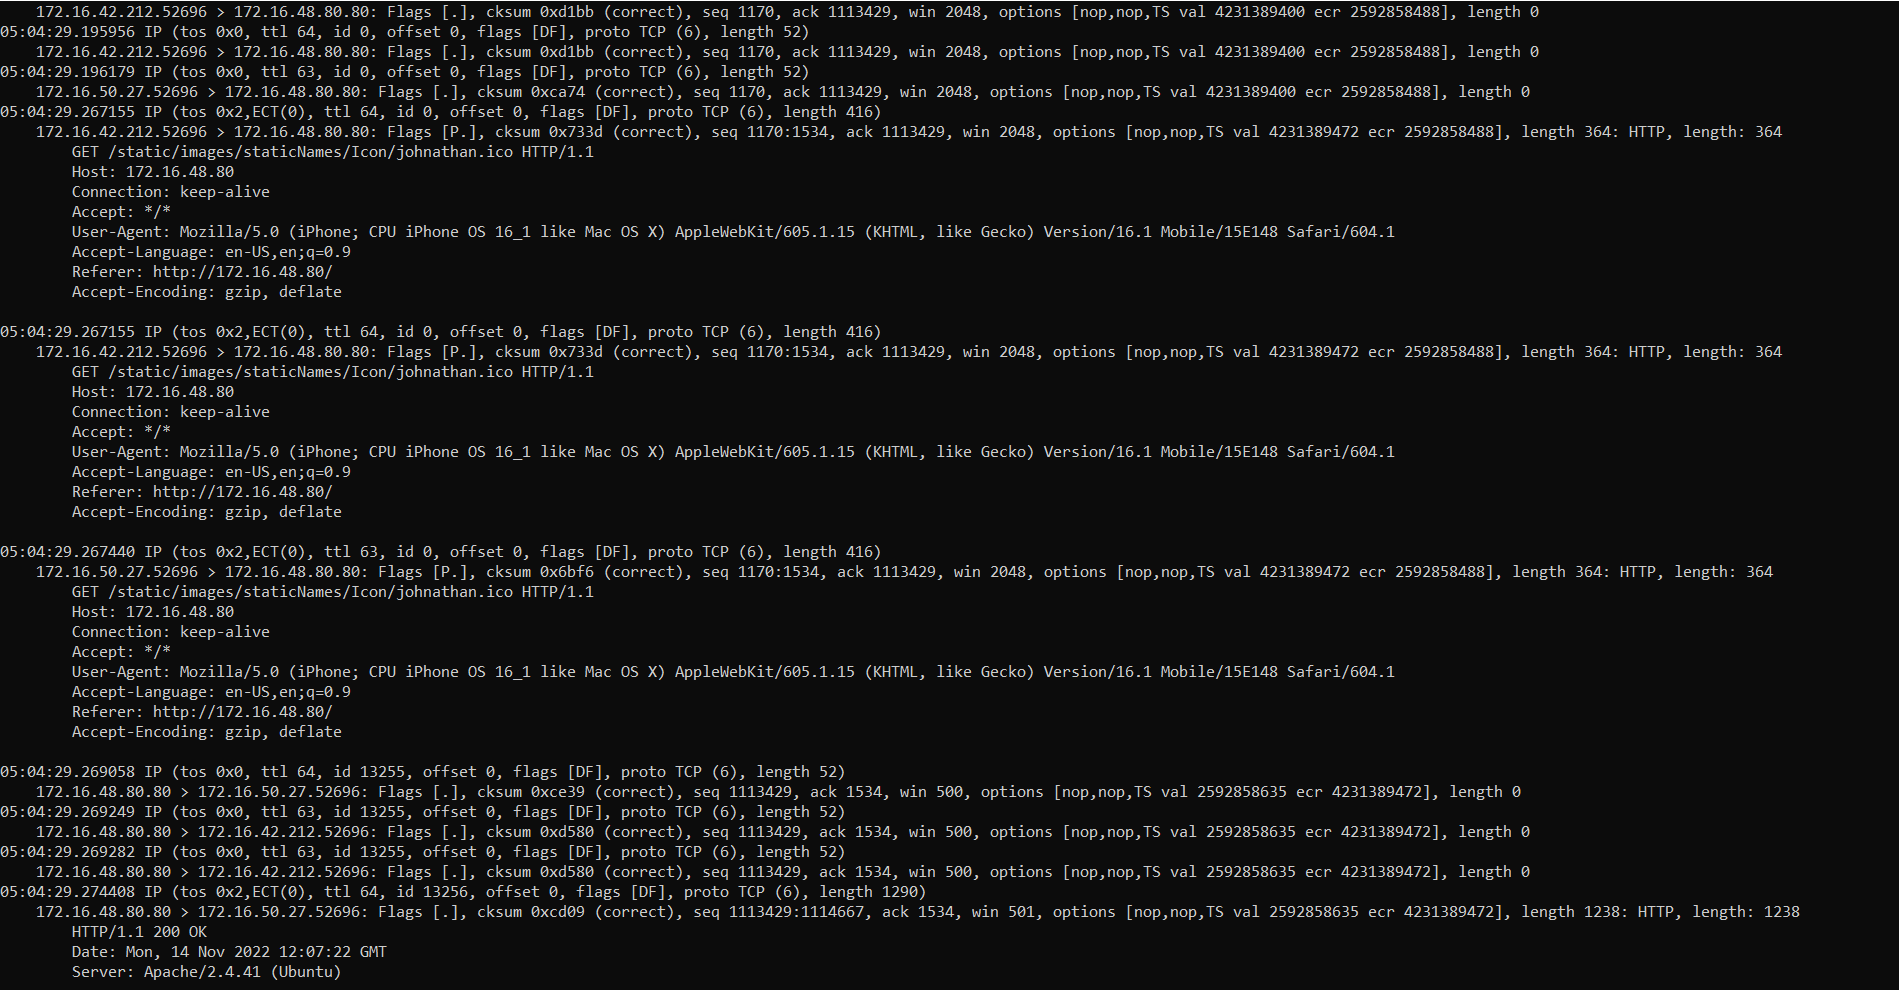
\includegraphics[width=1.0\textwidth]{assets/q5.png}
\end{align*}

$\hfill \break$
Notice however that the traffic looks pretty much the same as the previous capture from our vulnerable network. Principally, the security used to control who can get onto a network does not necessarily encrypt the traffic moving along that network. We can see this here, as the HTTP traffic is still visible in plaintext, and the only difference between the two captures is the IP addresses of the devices involved.

$\hfill \break$
In order to be able to hide the contents of the HTTP traffic being sent over the network, we would need to use HTTPS, which is a secure version of HTTP that encrypts the traffic using SSL/TLS. This is the same protocol that is used to encrypt traffic on the internet.

\newpage
\subsection*{Part 6}

We were able to detect all wireless APs in the lab when running the scan for this part of the lab, the results are shown below:

\begin{align*}
    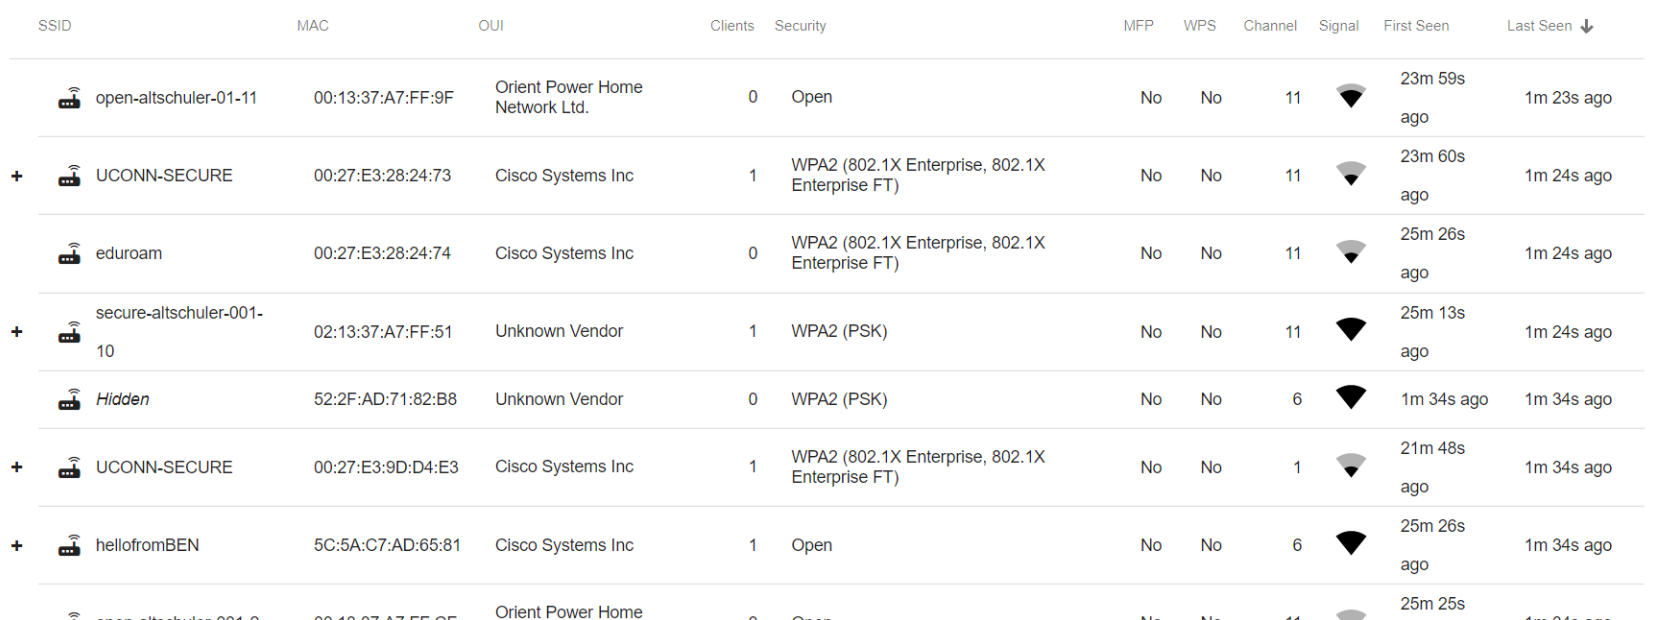
\includegraphics[width=1.0\textwidth]{assets/q6.png}
\end{align*}

$\hfill \break$
We were also able to identify some APs that announce more than one network due to the channel they were broadcasting. For example, in the above screenshot, we can see UCONN-SECURE twice, one with channel 11, and one with channel 1. This is because the AP is broadcasting on both channels, and the Pineapple is able to detect both of them.

$\hfill \break$
We can also see all of the different wireless security protocols being used by the APs in and around the lab. They were all either WPA2 (Enterprise). WPA2 (PSK), or Open. For some APs, we were able to see a client count, but it varied from 0 to 1, so we were not able to conclude how accurate this figure was.

\newpage
\subsection*{Part 7 and Part 8}

We were unable to complete these questions due to the number of active APs in the room interfering with each other.

\subsection*{Part 9}

\begin{enumerate}
    \item We were able to create the DNS records on the Pineapple to redirect requests to \textit{bank.com} and \textit{test.com} to the static IP address of our VM. This was accomplished by modifying the \textit{/etc/hosts} file as such:
    \begin{minted}[fontsize=\scriptsize]{bash}
127.0.0.1 localhost
172.16.51.49 bank.com
172.16.51.49 test.com

::1     localhost ip6-localhost ip6-loopback
ff02::1 ip6-allnodes
ff02::2 ip6-allrouters
    \end{minted}

    \item We were unable to complete this part due to the Pineapple not relaying the DNS configuration to our test machines.
\end{enumerate}

\end{document}
